\documentclass{article}

\usepackage{booktabs}
\usepackage{tabularx}
\usepackage{float}
\usepackage{graphicx} 
\usepackage{float} 
\usepackage{subfigure}
\usepackage[colorlinks,linkcolor=blue]{hyperref}

\title{Development Plan\\\progname}

\author{\authname}

\date{}

%% Comments

\usepackage{color}

\newif\ifcomments\commentstrue %displays comments
%\newif\ifcomments\commentsfalse %so that comments do not display

\ifcomments
\newcommand{\authornote}[3]{\textcolor{#1}{[#3 ---#2]}}
\newcommand{\todo}[1]{\textcolor{red}{[TODO: #1]}}
\else
\newcommand{\authornote}[3]{}
\newcommand{\todo}[1]{}
\fi

\newcommand{\wss}[1]{\authornote{blue}{SS}{#1}} 
\newcommand{\plt}[1]{\authornote{magenta}{TPLT}{#1}} %For explanation of the template
\newcommand{\an}[1]{\authornote{cyan}{Author}{#1}}

%% Common Parts

\newcommand{\progname}{Mechatronics} % PUT YOUR PROGRAM NAME HERE
\newcommand{\authname}{Team \#20, Team Name
\\ Robert Zhu zhul49
\\ Zifan Meng mengz17
\\ Jiahui Chen chenj194
\\ Kelvin Huynh huynhk12
\\ Runze Zhu zhur25
\\ Mirza Nafi Hasan hasanm21} % AUTHOR NAMES                  

\usepackage{hyperref}
    \hypersetup{colorlinks=true, linkcolor=blue, citecolor=blue, filecolor=blue,
                urlcolor=blue, unicode=false}
    \urlstyle{same}
                                


\begin{document}

\begin{table}[H]
\caption{Revision History} \label{TblRevisionHistory}
\begin{tabularx}{\textwidth}{llX}
\toprule
\textbf{Date} & \textbf{Developer(s)} & \textbf{Change}\\
\midrule
9/26/2022 & Everyone & Initial version\\

... & ... & ...\\
\bottomrule
\end{tabularx}
\end{table}

\newpage

\maketitle

\wss{Put your introductory blurb here.}

\section{Team Meeting Plan}

Team meetings are planned to occur after every 4TB6 lecture and during the lecture time if there is
no lecture on that day at the library or an alternative workspace. The team meeting is to be
organized three times a week and each meeting will be two to three hours in length depending on the
project deadlines and tasks. Meeting times are not completely fixed and more may be scheduled to accommodate
deadlines and the progress of the project.\\ There will be a meeting agenda for every meeting, and the agenda
will include the chair for that meeting, the planned tasks, final decision and take-home deliverables for
each team member. The chair for the meeting will be dependent on the content of the meeting. For example,
if the meeting is about hardware selection, the team member who is responsible for hardware component of the project
will be the chair for the meeting. 

\section{Team Communication Plan}

Team communication outside of meetings is to be conducted primarily on Facebook Messenger
for administrative related matters and project specifics. Communication relevant to the project
source code is encouraged to be conveyed through the use of Github Issues and\slash or Pull Requests
but may also be done through Facebook. In addition, communication to the relevant supervisor,
stakeholder, TA and\slash or course instructor will be conducted through the use of email.

\section{Team Member Roles}

As of now, every team member will have the same responsibilities consisting of coding,
identifying issues, testing, reviewing, and commenting on code. Further responsibilities
will include hardware-software integration and testing. More responsibilities will be
added as more specific tasks are discovered during the development process.

\begin{table}[H]
\caption{Roles and Responsibilities} \label{TblRoles}
\begin{tabularx}{\textwidth}{ll}
\toprule
\textbf{Name} & \textbf{Responsibilities}\\
\midrule
Robert Zhu & Coding, issue identification, testing, reviewing, and \\
Zifan Meng & commenting on code. Additionally hardware-software \\
Fred Zhu & integration. \\
Mirza Nafi Hasan & \\
Jiahui Chen & Research, hardware\\
Kelvin Huynh & \\
\bottomrule
\end{tabularx}
\end{table}

\section{Workflow Plan}

The Github and Gitlab will be used to manage the project. Before each modification, the new changes
must be pulled to make sure the working document is up to date for the master branch. Then, create
a new branch to work on the assigned tasks. The branch name should always reflect the content of the
tasks. For example, the branch name can be “updateGoals” when the goals need to be updated. After
the modification is finished in the branch, testing should be performed to ensure that no errors appear.
Then, the changes can be added, and merged into the master branch with a comment about the description
of the changes, and push the changes so that every team member can view the updated document.\\ Issues is
integrated with the GitHub repository and used to keep track of the current work. The issues template will
be created whenever a new issue type appears with the specific issue label like “bug”. And the future
issues with the same classification will use the existing issue template to create the issue.


\section{Proof of Concept Demonstration Plan}

Risks that can affect the success of the project include poor hand joint tracking
(which would have an effect on accuracy) and potentially a faulty machine learning model
that produces the incorrect results. Another risk would be that none of us have prior
knowledge of signing so that would affect the number of signable words and phrases that
we can use to further test validity and reliability of the machine learning model. During
the proof of concept demo, we hope to provide a mixture of basic signs and some complicated
signs such that we can see that we\textquotesingle re on the right track and that some part of the prototype
works. This will enable us to further refine our machine learning model and provide a
baseline that we can revert back to if it fails.

\section{Technology}

The coding for the project will be done in Python3 utilizing Flake8 as the linter
to ensure error-free and idiomatic code. Unit testing for the Python code will be done
through the use of the Pytest framework where various tests can be defined based on the
intended code functionality. The same framework of which can and will be used to generate
a measure of code coverage through the pytest-cov plugin. Continuous integration (CI) is
planned to be used to ensure that coding errors and bugs are detected within a reasonable
amount of time, however the specifics are to be determined as the group is unfamiliar with
implementing the concept at this time. Libraries that are currently planned for use include
OpenCV, Tensorflow, and Pyserial for serial communication with an Arduino board. Performance
measuring tools will be used appropriately as the need arises, but some examples would include
OpenCV\textquotesingle s getTickCount() and getTickFrequency() functions as well as Python\textquotesingle
s time.perf\textunderscore counter() function to track execution time of code. Additional tools
may be declared as the need arises.

\section{Coding Standard}

Code will loosely follow the \href{https://peps.python.org/pep-0008/}{PEP8 Python coding standard}.
The Flake8 linter will also ensure that written code will follow this standard.

\section{Project Scheduling}

\begin{figure}[H] 
\centering
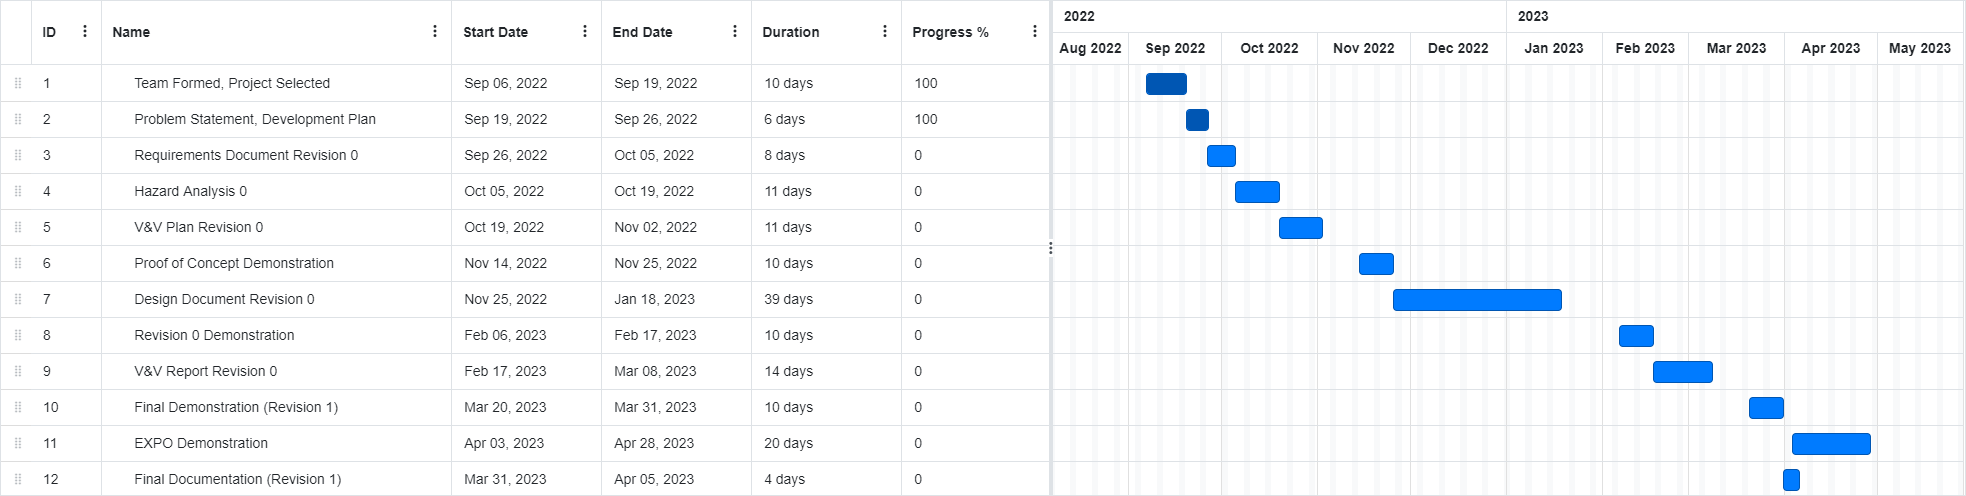
\includegraphics[width=1\textwidth]{Project Scheduling} 
\caption{Project Schedule} 
\label{Fig.Project_Scheduling} 
\end{figure}

Link to the updated Gantt Chart File is included
\href{https://drive.google.com/drive/folders/1M7_SSWqj6OOr_dPLmK_PLzeFSMWgSP8d?usp=sharing}{here}
.

\end{document}
